%! Author = noel.kempter
%! Date = 24.07.2022

\section{Google-Strategie}\label{sec:google-strategie}

In diesem Kapitel werfen wir einen kurzen Blick auf die Geschichte von Suchmaschinen und im Speziellen den Werdegang
von Google zur, mit Abstand, meist verwendeten Suchmaschine der Welt und der Strategie die das ermöglichte.

\subsection{Geschichte}\label{subsec:geschichte}
Die Geschichte der Suchmaschinen beginnt mit der Entstehung des Internets selbst Anfang der 90er Jahre.
Schon damals gab es unter den Suchmaschinen klare Favoriten, doch keiner davon hieß Google.
Die ersten großen Kompetitoren waren die Suchmaschinen AskJeeves, Lycos und Alta Vista, von denen heute keine mehr
Bestand als normale Suchmaschine hat.
Auch BackRub, entwickelt 1995 von den Google-Gründern Larry Page und Sergey Brin und daher von vielen als Vorgänger von
Google bezeichnet, konnte früh überzeugen hatte jedoch noch lange nicht solch eine dominante Marktstellung wie heute.
Wenig später kamen die auch heute noch relevanten Suchmaschinen Yahoo und MSN(2009 umbenannt in Bing) mit
ins Rennen.
Heute teilen sich Google, Yahoo und Bing je nach Region insgesamt bis zu 95\% der Marktanteile, wobei Google stets
mindestens ein 7-faches der Marktanteile aller Mitbewerber gemeinsam ausmacht.

\subsection{Google Strategie}\label{subsec:google-strategie}
Dazu kommen konnte es dank der außergewöhnlichen Unternehmensstrategie von Google, welche sich auf verschiedene Grundlagen
stützt.
Ein Aspekt des Erfolges von Google ist die Innovativität.
Schon in den Anfangstagen der Suchmaschine konnte diese durch innovatives Design und Ideen, welche zu schnelleren und
besseren Suchergebnissen führte überzeugen.
So war es Google welche mit dem PageRank zum ersten Mal eine Bewertungsskala für Webseiten anlegte und aktiv in die
Anzeige von Suchergebnissen mit einbezog.
Dieses Ranking-Schema bewerte Webseiten nicht nur anhand des Inhalts, sondern unter anderem auch an der Anzahl
eingehender Links einer Seite, der Qualität der Seiten von denen diese Links kommen, dem Layout beziehungsweise Design
der Seite bewertet nach W3C-Kriterien und vielen weiteren Faktoren.
Damit konnte Google schon Ende der 90er Jahre qualitativ hochwertigere Suchergebnisse liefern als alle Konkurrenten.
Ein weiterer Erfolgsaspekt ist das Design der Seite dem bis zum heutigen Tage treu geblieben wird.
Was heute als eher schlicht, teilweise schon langweilig, empfunden werden könnte hatte in den frühen Tagen des Internets
klare Vorteile, welche mit zum Sieg über die Mitbewerber beitrugen.
Denn während Bing, Yahoo und andere Konkurrenten ihre Seiten zu Webportalen weiterentwickelten, auf denen neben der
Suchmöglichkeit auch aktuelle Nachrichten, dass Wetter und weitere Informationen zu sehen waren, blieb Goggle dem schlichten
Design treu, was aufgrund der damals noch stark begrenzten Ressourcen in Sachen Rechenleistung und Internetgeschwindigkeit
zu deutlich schnelleren Ladezeiten als bei den Mitbewerbern und damit einer besseren User-Experience führte.
Außerdem konnte Google seinen Index, das heißt die Anzahl der bekannten und vernetzten Seiten schneller ausbauen als die
Konkurrenten und zur Jahrtausendwende mit über einer Milliarde bekannten Webdokumenten zur größten Suchmaschine der Welt.
Des Weiteren führte die Einführung von GoogleAdWords, einem Service welcher es Kunden ermöglicht ihre Werbung an
bestimmte Suchbegriffe zu koppeln und gemeinsam mit den eigentlichen Suchergebnissen anzeigen zu lassen, im Jahr 2000 und
der Börsengang im Jahr 2004 zu massiven Geldeinnahmen und dem Wunsch vieler an diesem Erfolg Teil zu haben.
Doch anstatt sich auf diesem Erfolg auszuruhen wurden diese Einnahmen verwendet, um die Marktpalette des Internetgiganten
zu erweitern, wodurch dieser den Konkurrenten abermals einen Schritt voraus war.
So wurden in den Jahren 2004/2005, dem Zeitraum in dem Google alle Konkurrenten endgültig zurückließ, die Dienste Google Mail,
Google Maps und Google Earth in Betrieb genommen.
Während es für die beiden letzteren Dienste aufgrund der Neuartigkeit dieser Technologien kaum ernst zu nehmende
Konkurrenz gab, war ein E-Mail-Service mitte der 2000er längst nichts Ungewöhnliches mehr.
Was Gmail jedoch auszeichnete und letzten Endes zum Erfolg verhalf, war die damalige Größe des Postfachs von einem
Gigabyte Speicher, welcher die Konkurrenten, deren Postfächer meist auf zwei bis höchstens zwanzig Megabyte beschränkt
waren, um das fünfzig- bis sogar fünfhundertfache übertrumpfte.
Auch durch das behutsam gepflegte Firmenimage gepaart mit Gags und Events um die Nutzer zu belustigen kann
die Suchmaschine überzeugen.
So kommt das auf der Startseite angezeigte Firmenlogo, wie in Abbildung ~\ref{fig:google_doodle} zu erkennen, je nach Anlass in
unterschiedlicher Aufmachung daher und auch Easter Eggs, das heißt versteckte Funktionen, die keinen wirklichen Sinn haben,
sind in der Suchmaschine verbaut(wer so etwas noch nicht kennt, muss in der Sucheingabe nur einmal \('\)do a barrel roll' eingeben)
und machen das Surfen zu einer waren Experience.
Als letzten Grund für den Erfolg der Suchmaschine, auf den in diesem Werk eingegangen wird, sind die exzellenten
Akquisitionen anderer Unternehmen zu nennen wie unter anderem Android im Jahr 2005 und YouTube 2006.
Diese ermöglichten es neue Märkte zu erschließen und den Einfluss des Unternehmens im Netz massiv auszubauen.

\begin{figure}[ht]
    \centering
    \fbox{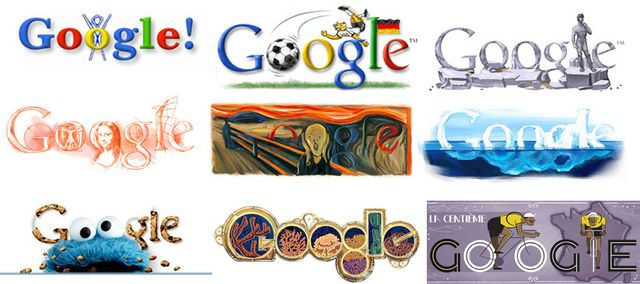
\includegraphics[height=0.3\textheight]{google_doodles}}\caption{Google Doodles}\label{fig:google_doodle}
\end{figure}

\subsection{Zusammenfassung}\label{subsec:zusammenfassung}
Die oben erläuterten Gründe sind nur einige derer, die aus Google die mit Abstand meist verwendete Suchmaschine der Welt
machten.
Doch wie auch seine Vorgänger ist Google alles andere als frei von Fehlern und könnte in Zukunft möglicherweise durch einen
neuen und besser an die Bedürfnisse der Nutzer angepassten Mitbewerber abgelöst werden.